%% CAPE-EEG manuscript for NSysS 2026 (ACM sigconf). Build: tectonic submission.tex (double-blind, <= 8 pages)
%% or tectonic camera.tex (author version with appendix, <= 9 pages). Numbers for the post-lock development
%% analyses are generated into numbers.tex by multiseed_ablation.py.
\ifdefined\ANONYMOUS
  \documentclass[sigconf,anonymous]{acmart}
\else
  \documentclass[sigconf]{acmart}
\fi
\usepackage{booktabs}
\usepackage{subcaption}
\usepackage{tikz}
\usetikzlibrary{positioning,arrows.meta,shapes.geometric,calc,fit,backgrounds}
\usepackage{xcolor}
\usepackage{pifont}
\emergencystretch=2.5em
\hyphenation{pre-speci-fied spectro-gram spectro-grams para-meters annota-tor annota-tors calibra-tion re-pro-duc-ible}
\settopmatter{printacmref=false}
\setcopyright{none}
\renewcommand\footnotetextcopyrightpermission[1]{}
\acmConference[NSysS '26]{13th International Conference on Next Generation Computing, Communication, Systems and Security}{December 17--19, 2026}{Cox's Bazar, Bangladesh}
\acmYear{2026}
\copyrightyear{2026}
\acmDOI{}
\acmISBN{}
% generated by multiseed_ablation.py; do not edit
\newcommand{\klAone}{0.976}
\newcommand{\sdAone}{0.037}
\newcommand{\nAone}{3}
\newcommand{\klAtwo}{0.979}
\newcommand{\sdAtwo}{0.015}
\newcommand{\nAtwo}{3}
\newcommand{\klBtwo}{0.979}
\newcommand{\sdBtwo}{0.016}
\newcommand{\nBtwo}{3}
\newcommand{\klBthree}{0.913}
\newcommand{\sdBthree}{0.028}
\newcommand{\nBthree}{3}
\newcommand{\klBthreeH}{1.088}
\newcommand{\sdBthreeH}{0.024}
\newcommand{\nBthreeH}{3}
\newcommand{\klBthreeS}{1.103}
\newcommand{\sdBthreeS}{0.077}
\newcommand{\nBthreeS}{3}
\newcommand{\klP}{0.990}
\newcommand{\sdP}{0.063}
\newcommand{\nP}{3}
\newcommand{\dfoveation}{-0.002}
\newcommand{\dsdfoveation}{0.038}
\newcommand{\dgate}{+0.002}
\newcommand{\dsdgate}{0.052}
\newcommand{\daux}{+0.012}
\newcommand{\dsdaux}{0.048}
\newcommand{\dall}{+0.012}
\newcommand{\dsdall}{0.072}
\newcommand{\dpretrain}{-0.190}
\newcommand{\dsdpretrain}{0.068}
\newcommand{\dwidth}{-0.175}
\newcommand{\dsdwidth}{0.052}
\newcommand{\dbthreevsbtwo}{-0.066}
\newcommand{\dsdbthreevsbtwo}{0.017}
\newcommand{\dpvsbthree}{+0.078}
\newcommand{\dsdpvsbthree}{0.067}
\newcommand{\dscratchvsp}{+0.113}
\newcommand{\dsdscratchvsp}{0.031}
\newcommand{\dhalfvsp}{+0.097}
\newcommand{\dsdhalfvsp}{0.068}
\newcommand{\testpairedsd}{0.329}
\newcommand{\testmde}{0.047}
\newcommand{\ntestpat}{391}


\definecolor{cblue}{HTML}{1F77B4}
\definecolor{corange}{HTML}{E8710A}
\definecolor{cgreen}{HTML}{2CA02C}
\definecolor{cgrey}{HTML}{F2F2F2}
\newcommand{\kl}{\mathrm{KL}}
\newcommand{\ci}[2]{[#1,\,#2]}
\newcommand{\yes}{\ding{51}}
\newcommand{\no}{--}
\newcommand{\nr}{n/r}
\ifdefined\ANONYMOUS\newcommand{\learningref}{}\newcommand{\paretoref}{}\newcommand{\alignref}{ (audited with a synthetic impulse; figure in the supplement)}\else\newcommand{\learningref}{ and Figure~\ref{fig:learning}}\newcommand{\paretoref}{ (Figure~\ref{fig:pareto})}\newcommand{\alignref}{ (Figure~\ref{fig:align})}\fi
\ifdefined\ANONYMOUS
  \newcommand{\repourl}{an anonymised repository}
\else
  \newcommand{\repourl}{\url{https://github.com/Hisernberg/cape-eeg}}
\fi

\begin{document}

\title[When Compact Is Not Enough: Protocol-Locked Evaluation of CAPE-EEG]{When Compact Is Not Enough: A Protocol-Locked, Resource-Bounded Evaluation of CAPE-EEG for Expert-Vote Classification of Harmful Brain Activity}

\author{Nabid Nur}
\affiliation{%
  \institution{Independent Researcher}
  \city{Dhaka}
  \country{Bangladesh}}
\renewcommand{\shortauthors}{Nur}

\begin{abstract}
Intensive-care EEG produces expert labels that disagree, so a useful classifier must estimate the distribution of expert opinion, stay calibrated, know when to defer, and remain auditable on modest hardware. We ask whether a 164k-parameter two-view convolutional model, CAPE-EEG, can match a small ImageNet-pretrained network when both consume the same byte-capped evidence. Each labelled 10-second window is encoded as a \emph{foveated} log-spectrogram of the surrounding 50-second raw EEG (half of the 32 time bins on the labelled centre) and a 64$\times$64 summary of the supplied 10-minute spectrogram, stored as float16 with bit-packed validity masks in a 5.58\,GB cache. CAPE-EEG fuses the views with a learned gate and predicts observed annotator disagreement as an auxiliary target. On 106,800 windows from 1,950 patients of the HMS Harmful Brain Activity dataset we froze a patient-disjoint 60/10/5/5/20 split, capped development at eight named configurations, locked the comparator, schedule and referral score in a hashed protocol document before any held-out access, and scored the test partition once. The hypothesis is falsified: three-seed patient-mean KL divergence is 0.934 for CAPE-EEG versus 0.869 for MobileNetV3-Small on identical inputs (paired difference $+0.066$, 95\% patient-bootstrap CI $\ci{+0.033}{+0.097}$, 391 patients). Post-lock three-seed development ablations under the frozen schedule show that foveation, the learned gate and the disagreement loss each change tune loss by less than the seed-to-seed spread, and that the comparator's advantage is a transfer-learning effect: trained from scratch, or at half width with ImageNet weights, MobileNetV3-Small falls 0.11 and 0.10 KL \emph{behind} the compact model. The audits are the durable contribution: temperature scaling removes over-confidence in both families, entropy-based deferral lowers accepted-case risk, evidence deletion confirms that the compact model relies on the labelled raw-EEG window, and the two families have different failure surfaces, with the pretrained network three times more sensitive to a change of STFT resolution. The locked study used 0.72 GPU-hours on one desktop accelerator (1.08 with the post-lock analyses); code, 155 tests, executed notebooks, the protocol document and twenty provenance-tracked figures are released.
\end{abstract}

\begin{CCSXML}
<ccs2012>
<concept><concept_id>10010147.10010257</concept_id><concept_desc>Computing methodologies~Machine learning</concept_desc><concept_significance>500</concept_significance></concept>
<concept><concept_id>10010405.10010444.10010449</concept_id><concept_desc>Applied computing~Health informatics</concept_desc><concept_significance>300</concept_significance></concept>
<concept><concept_id>10002944.10011122.10002945</concept_id><concept_desc>General and reference~Reliability</concept_desc><concept_significance>300</concept_significance></concept>
</ccs2012>
\end{CCSXML}
\ccsdesc[500]{Computing methodologies~Machine learning}
\ccsdesc[300]{Applied computing~Health informatics}
\ccsdesc[300]{General and reference~Reliability}
\keywords{EEG, harmful brain activity, soft labels, expert disagreement, compact neural networks, protocol-locked evaluation, calibration, robustness, resource-bounded machine learning}

\maketitle

\section{Introduction}
Continuous EEG in intensive care is read for seizures and for the rhythmic and periodic patterns that surround them: lateralised and generalised periodic discharges (LPD, GPD) and lateralised and generalised rhythmic delta activity (LRDA, GRDA). Expert readers disagree about these patterns, and the largest public dataset of such annotations, HMS Harmful Brain Activity Classification, therefore scores a model against the \emph{vote distribution} of up to 28 experts with the Kullback--Leibler divergence rather than against a single label \cite{hms2024,jing2023}. This changes what a good model is: it must be calibrated, it must know when to defer, and its use of evidence must be inspectable, because the reference itself is a disagreement.

Systems that would run such models beside a monitor are constrained in ways that leaderboard solutions are not: bounded memory and storage, one shared small accelerator, and a requirement that every trained artefact be reproducible and inspectable. Two ideas from recent computer vision seem tailored to this regime. Foveated representations spend resolution where the label lives \cite{akbas2017foveated}, and economical multi-scale fusion combines views without a large backbone \cite{kang2026dpnext}. Recent EEG work adds four warnings: preprocessing choices silently move predictions \cite{hou2026samebrain}; foundation models are not automatically better than task-matched controls \cite{kontras2026neuroatlas}; purported evidence should be tested by deletion \cite{wang2026evidence}; and robustness must be measured under declared perturbations \cite{mohammadi2026robustseiz}.

This paper is not a leaderboard entry. Strong HMS systems such as VIPEEGNet \cite{sun2025vipeegnet} reach external KL near 0.22--0.27 on the competition's high-agreement test set with a 12.9M-parameter pretrained backbone and ensembling; our KL is computed over \emph{every} labelled window of a patient-disjoint split, including single-annotator windows, and is not comparable to those figures. Our question is narrower and falsifiable: under a strict, resource-bounded protocol, does a compact, evidence-selective, auditable architecture retain the discrimination of a small pretrained CNN that sees exactly the same bytes?

We answer four research questions:
\begin{itemize}
\item \textbf{RQ1 (primary).} At a fixed cache byte budget and a bounded single-device training budget, does CAPE-EEG beat the small comparator selected on tuning data, measured by three-seed patient-mean KL on a locked, patient-disjoint test partition?
\item \textbf{RQ2 (mechanisms).} Do temporal foveation, a learned view gate and a disagreement auxiliary loss each improve loss at identical bytes, trunk, schedule and augmentation, by more than ordinary seed variation?
\item \textbf{RQ3 (confounds).} Is the comparator's advantage explained by ImageNet pretraining or by its nine-fold larger parameter count?
\item \textbf{RQ4 (audits).} What do calibration, deferral, evidence-deletion and corruption audits reveal that the headline KL hides, and do the two model families fail in the same way?
\end{itemize}

Our contributions are: (1) a protocol-locked, leak-free evaluation design for expert-vote EEG classification with a patient/recording connected-component split, a 6\,GB active-cache cap that counts masks and metadata, at most eight named development configurations, three fixed seeds averaged as losses, and a single scored held-out evaluation with patient-cluster bootstrap inference \cite{nosek2018preregistration,efron1979bootstrap}; (2) CAPE-EEG, a 164k-parameter two-view model with byte-matched temporal foveation, an inspectable learned view gate and an annotation-disagreement head, released with its exact byte- and exposure-matched controls; (3) a resolved negative answer to RQ1 and three-seed answers to RQ2 and RQ3 obtained without touching the test partition again; (4) audits that survive the negative result, with patient-cluster intervals throughout; and (5) an open, tested release (155 synthetic tests, seven executed notebooks, the verbatim protocol document and twenty figures with provenance sidecars) at \repourl. Table~\ref{tab:position} positions the study against the work it builds on.

\begin{table*}[t]
\caption{Positioning against related work. \yes{} = present and reported; \no{} = absent by design or not applicable; \nr{} = not reported in the cited description. Rows describe the cited papers as published, not their authors' capabilities.}
\label{tab:position}
\footnotesize
\setlength{\tabcolsep}{5pt}
\renewcommand{\arraystretch}{0.92}
\newcommand{\hd}[1]{\begin{tabular}[c]{@{}c@{}}#1\end{tabular}}
\resizebox{\textwidth}{!}{%
\begin{tabular}{llcccccccc}
\toprule
Study & Task & \hd{Patient-disjoint\\split} & \hd{Byte-matched\\controls} & \hd{Locked\\protocol} & \hd{Soft-label\\KL} & \hd{Separate\\calibration set} & \hd{Deferral\\analysis} & \hd{Evidence\\deletion} & \hd{Declared\\corruption suite} \\
\midrule
VIPEEGNet \cite{sun2025vipeegnet} & HMS 6-class & \nr & \no & \nr & \yes & \nr & \nr & \nr & \nr \\
Evidence bottleneck \cite{wang2026evidence} & EEG diagnosis & \nr & \no & \nr & \no & \nr & \nr & \yes & \nr \\
RobustSeiz \cite{mohammadi2026robustseiz} & seizure detection & \yes & \no & \nr & \no & \nr & \nr & \nr & \yes \\
NeuroAtlas \cite{kontras2026neuroatlas} & multi-task EEG & \yes & \no & \nr & \no & \nr & \nr & \nr & \nr \\
Preprocessing reliability \cite{hou2026samebrain} & EEG decoding & \yes & \no & \nr & \no & \nr & \nr & \nr & \yes \\
\textbf{This work} & HMS 6-class & \yes & \yes & \yes & \yes & \yes & \yes & \yes & \yes \\
\bottomrule
\end{tabular}}
\end{table*}

\section{Related Work}
\textbf{HMS and vision-inspired classifiers.} Jing et al.\ \cite{jing2023} showed that a deep model can reach expert-level agreement on the six-pattern task, and the public HMS release \cite{hms2024} operationalised the task as vote-distribution prediction scored by KL. VIPEEGNet \cite{sun2025vipeegnet}, published in \emph{npj Digital Medicine}, adapts an ImageNet-pretrained backbone to spectrogram images and reports external KL of 0.223 and 0.273, among the best of 2,767 competition entries, with 2.8\% of the parameters of the top entry. Its scores are computed on the competition's test protocol, whose windows are weighted towards high annotator agreement, and its cohort construction differs from ours, so they anchor the field rather than our table. Our comparator B3 is the smallest member of that family, MobileNetV3-Small \cite{howard2019mobilenetv3}, chosen so that the comparison is about representation rather than scale.

\textbf{Compact architectures and fusion.} Depthwise-separable convolutions \cite{howard2017mobilenets} and Group Normalisation \cite{wu2018groupnorm} make sub-200k-parameter trunks trainable at small batch sizes. DPNeXt \cite{kang2026dpnext} shows that inexpensive multi-scale fusion can replace heavy decoders in dense prediction; we borrow only the principle as an exploratory block and find it harmful here.

\textbf{Soft labels, calibration and deferral.} Learning from the full distribution of human judgements improves robustness and calibration \cite{peterson2019human}; temperature scaling \cite{guo2017calibration} is the minimal post-hoc calibrator we allow, fitted on a partition that never trains weights. Selective classification \cite{geifman2017selective} motivates the risk--coverage analysis in which a frozen input-only score decides which windows to refer.

\textbf{Reliability of EEG decoding.} The preprocessing-sensitivity, benchmark, evidence-bottleneck and robustness studies of 2026 \cite{hou2026samebrain,kontras2026neuroatlas,wang2026evidence,mohammadi2026robustseiz} motivate, respectively, our declared STFT-resolution condition, our task-matched controls, our deletion audits and our corruption suite. None is reproduced; each is the reason a specific test exists.

\section{Data and Task}
\label{sec:data}
The source is the original HMS training release: 106,800 labelled windows from 1,950 patients, 17,089 EEG recordings (200\,Hz, 19 scalp electrodes plus EKG, 50\,s to 56\,min long) and 11,138 spectrograms (2\,s rows, four regions $\times$ 100 frequencies from 0.59 to 19.92\,Hz). Each row gives an EEG offset $e$ and a spectrogram offset $s$; the labelled centre is seconds $[e{+}20,e{+}30)$ of the recording and $[s{+}295,s{+}305)$ of the spectrogram, and the two clocks differ \cite{hms2024}. Votes $v_{ik}\ge 0$ over six classes have totals $n_i\in[1,28]$; 4,360 windows carry a single vote and 5,248 have tied maxima. The target is $q_{ik}=v_{ik}/n_i$. The prediction unit is a window; the independence unit is the patient, and because no recording is shared across patients the 1,950 connected components coincide with patients. Table~\ref{tab:partitions} gives the deterministic allocation, which balanced rows, per-class vote mass and component counts without consulting any model.

\begin{table}[t]
\caption{Frozen partitions (patient/recording components, seed 20260907). No patient, EEG or spectrogram appears in two partitions.}
\label{tab:partitions}
\small
\setlength{\tabcolsep}{4pt}
\begin{tabular}{lrrrl}
\toprule
Partition & Rows & Patients & Share & Role \\
\midrule
Train & 64,292 & 1,170 & 0.602 & development fits \\
Tune & 10,667 & 196 & 0.100 & comparator, epochs, score \\
Calibration-T & 5,289 & 95 & 0.050 & temperature only \\
Calibration-P & 5,247 & 98 & 0.049 & referral thresholds \\
Locked test & 21,305 & 391 & 0.200 & one scored evaluation \\
\bottomrule
\end{tabular}
\end{table}

\section{CAPE-EEG}
\subsection{Byte-budgeted two-view evidence}
\label{sec:cache}
Every window becomes two float16 tensors. The \textbf{local view} $L\in\mathbb{R}^{4\times 64\times 32}$ comes from the 50\,s raw window: sixteen bipolar leads in four regional chains (LL, RL, LP, RP), per-lead median removal, a Hann STFT (256-sample window, hop 64, 153 frames), linear power averaged over the valid leads of a region, overlap-weighted integration into 64 linear frequency bins over 0.5--40\,Hz and 32 time bins, then a logarithm. The \emph{foveated} encoding covers $[0,20)$\,s with 8 bins, the labelled centre $[20,30)$\,s with 16 bins and $[30,50)$\,s with 8 bins; the \emph{uniform} control uses 32 equal bins, at exactly the same bytes\alignref. The \textbf{context view} $C\in\mathbb{R}^{4\times 64\times 64}$ integrates the supplied 600\,s spectrogram interval onto 64 frequency and 64 time bins per region. Each cell carries a validity bit: a frame needs at least 90\% observed samples and two valid leads, a bin at least half of its weight from valid frames; non-finite supplied cells are invalid; truncated edges are masked, never shifted. One row occupies 49,152 bytes of values and 3,072 bytes of masks; the realised cache holds 106,800 rows in 5.582\,GB, under the 6\,GB cap, plus a 1.859\,GB development-only uniform alternate. Float16 storage changes log-power by at most 0.0076. Conversion took 786\,s with 16 CPU workers whose resident memory stayed below 0.77\,GiB.

\ifdefined\ANONYMOUS\else
\begin{figure}[t]
\centering
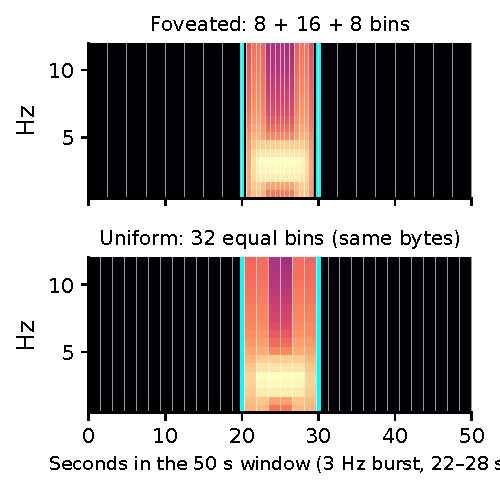
\includegraphics[width=0.92\linewidth]{figures/fig_alignment.pdf}
\caption{Alignment audit that every cache must pass: a synthetic 3\,Hz burst confined to seconds 22--28 through the real encoder. Foveated bins are drawn with their true widths (white lines); the labelled centre $[20,30)$\,s is marked in cyan. The uniform control spends the same bytes with equal bins.}
\label{fig:align}
\end{figure}
\fi

\subsection{Architecture}
\begin{figure}[t]
\centering
\begin{tikzpicture}[x=1mm, y=1mm, font=\footnotesize, >={Stealth[length=4pt]},
  box/.style={draw, rounded corners=2pt, fill=cgrey, minimum height=5mm, inner sep=2.5pt, align=center},
  view/.style={box, fill=cblue!15}, head/.style={box, fill=corange!18}, gate/.style={box, fill=cgreen!18}]
\node[view, text width=32mm] (L) at (-19,0) {local view $L$\\$4{\times}64{\times}32$};
\node[view, text width=32mm] (C) at (19,0) {context view $C$\\$4{\times}64{\times}64$};
\node[box, text width=32mm] (sL) at (-19,-9) {stem$_L$: 3$\times$3, 4$\to$24};
\node[box, text width=32mm] (sC) at (19,-9) {stem$_C$: 3$\times$3, 4$\to$24};
\node[box, text width=72mm] (trunk) at (0,-20) {\textbf{shared trunk}: depthwise-separable blocks, GroupNorm, channels 24$\to$48$\to$64$\to$96$\to$128, strides (2,1),(2,2),(2,2),(1,1), two residual blocks};
\node[box, text width=34mm] (pL) at (-19,-32) {pool mean $\|$ max $\|$ centre$_w$\\projection $\to u_L\in\mathbb{R}^{128}$};
\node[box, text width=34mm] (pC) at (19,-32) {pool mean $\|$ max\\projection $\to u_C\in\mathbb{R}^{128}$};
\node[head, text width=22mm] (hL) at (-19,-42) {head$_L$ $\to p_L$};
\node[head, text width=22mm] (hC) at (19,-42) {head$_C$ $\to p_C$};
\node[gate, text width=72mm] (g) at (0,-52) {gate $g=\sigma(\mathrm{MLP}[u_L,u_C,\text{valid}_L,\text{valid}_C,\mathrm{JS}(p_L,p_C)])$\\mixture $p=(1-g)\,p_L+g\,p_C$; a missing view forces $g\in\{0,1\}$};
\node[head, text width=72mm] (aux) at (0,-62) {disagreement head $\hat d=\sigma(\mathrm{MLP}[u_L,u_C])$, supervised in training only (weight 0.1)};
\draw[->] (L)--(sL); \draw[->] (C)--(sC);
\draw[->] (sL.south)--(trunk.north -| sL.south); \draw[->] (sC.south)--(trunk.north -| sC.south);
\draw[->] (trunk.south -| pL.north)--(pL.north); \draw[->] (trunk.south -| pC.north)--(pC.north);
\draw[->] (pL)--(hL); \draw[->] (pC)--(hC);
\draw[->] (hL.south)--(g.north -| hL.south); \draw[->] (hC.south)--(g.north -| hC.south);
\draw[->, dashed] (pL.east) -- ++(6,0) |- (aux.west);
\end{tikzpicture}
\caption{CAPE-EEG (164,134 parameters). The centre-weighted pool uses the true bin edges of the encoding in use, so the uniform control pools its real centre. Ablations remove the gate (fixed 50:50), the auxiliary head, or the foveation; no identifier, vote count or label enters the network at inference.}
\label{fig:arch}
\end{figure}

Figure~\ref{fig:arch} shows the candidate. Each view has its own $3\times 3$ stem and both share a depthwise-separable trunk with 24, 48, 64, 96 and 128 channels, frequency/time strides of (2,1), (2,2), (2,2) and (1,1), and two residual 128-channel blocks; GroupNorm avoids batch statistics. Local pooling concatenates the global mean, the global maximum and a centre-region mean whose column weights are the overlap of each bin with $[20,30)$\,s. Context pooling uses mean and maximum. Linear projections give $u_L,u_C\in\mathbb{R}^{128}$ and independent heads give $p_L$ and $p_C$. The gate sees the two embeddings, the two valid fractions and the Jensen--Shannon divergence between $p_L$ and $p_C$. Heads, gate and mixture run in float32 even under bf16 autocast.

\subsection{Losses}
The classification loss is the soft cross-entropy $-\sum_k q_{ik}\log p_{ik}$ on the mixture, whose optimum equals that of $\kl(q_i\|p_i)$. Observed pairwise annotator disagreement $d_i=1-\sum_k v_{ik}(v_{ik}-1)/[n_i(n_i-1)]$ is defined for $n_i>1$ and not clipped to its population maximum of $5/6$; the total loss is $\overline{\mathrm{CE}}+0.1\cdot\overline{(\hat d_i-d_i)^2}_{\,n_i>1}$ with a differentiable zero when a mini-batch has no multi-annotator window. We note for RQ2 that $d_i$ is a finite-sample function of the same vote vector that defines $q_i$ (for large $n_i$ it approaches $1-\sum_k q_{ik}^2$), so the auxiliary target is correlated with, though not identical to, the primary target; Section~\ref{sec:ablation} tests whether it still helps. No class weighting, vote weighting, focal loss or label sharpening is used.

\subsection{Baselines and named configurations}
\label{sec:configs}
B0 is the training-set vote prior; B1 is an L2-regularised multinomial logistic regression on 74 fixed band-power features fitted to fractional targets on the CPU. Eight named GPU configurations were permitted in development. B2 is the byte-matched control: the same trunk on the uniform encoding with a fixed 50:50 mixture and no auxiliary head (147,524 parameters). A1 adds foveation, A2 the learned gate, P the auxiliary loss. B3 is MobileNetV3-Small \cite{howard2019mobilenetv3,wightman2019timm} with four input channels and six outputs, fed the two normalised views concatenated along time (64$\times$96) and bilinearly resized to 128$\times$192 (1,524,150 parameters). P+MSF replaces the last residual block of P by an economical multi-scale fusion block (parallel depthwise convolutions with temporal dilations 1/2/3, a $1\times 1$ fusion and a channel gate; 208,070 parameters). The seventh and eighth named configurations, P$_3$ and B3$_3$, are P and B3 under a complete 3-epoch cosine schedule (Section~\ref{sec:dev}). B0 and B1 need no GPU and were not counted against the cap; the permitted $0.3\times$ learning-rate pilot was not used. Only B2 and B3 were eligible to become the comparator, chosen on tune data.

\subsection{Training}
All configurations use AdamW \cite{loshchilov2019adamw} (weight decay 0.01), learning rate $10^{-3}$ for compact models and $10^{-4}$/$10^{-3}$ for pretrained backbone/head with one frozen-backbone epoch, cosine decay with 200 warm-up steps, batch 64, gradient clipping at 1.0, bf16 autocast after a parity test (maximum $|\Delta p|=0.005$), and mild augmentation only: Gaussian gain jitter, frequency masking of at most four bins, and single-region dropout with probability 0.1. Normalisation statistics (median and scaled MAD of valid cells per view and region) are fitted on the training partition only and refitted on train+tune for the final phase; invalid cells are zeroed after normalisation.

\section{Protocol-Locked Evaluation}
\label{sec:protocol}
\begin{figure*}[t]
\centering
\resizebox{\textwidth}{!}{%
\begin{tikzpicture}[
  font=\footnotesize, >={Stealth[length=4pt]}, node distance=2.2mm and 3mm,
  st/.style={draw, rounded corners=2pt, fill=cgrey, minimum height=10mm, text width=27mm, align=center, inner sep=2pt},
  dev/.style={st, fill=cblue!14}, lock/.style={st, fill=corange!22, draw=corange!80!black, thick}, fin/.style={st, fill=cgreen!16}]
\node[st] (a) {\textbf{source audit}\\schema gate, checksums, offset-grid and alignment tests};
\node[st, right=of a] (b) {\textbf{component split}\\60/10/5/5/20, seed fixed, 5$\times$5 overlap = 0};
\node[st, right=of b] (c) {\textbf{byte-capped cache}\\float16 + packed masks, 5.58\,GB $\le$ 6\,GB};
\node[dev, right=of c] (d) {\textbf{development}\\8 named configs, train $\to$ tune only};
\node[lock, right=of d] (e) {\textbf{protocol lock}\\comparator, schedule, referral score, strata, figures};
\node[fin, right=of e] (f) {\textbf{final refits}\\train+tune, 3 seeds, complete schedule};
\node[fin, right=of f] (g) {\textbf{calibration}\\$T$ on Cal-T; thresholds on Cal-P};
\node[lock, right=of g] (h) {\textbf{locked test}\\one scored evaluation; paired bootstrap};
\draw[->] (a)--(b); \draw[->] (b)--(c); \draw[->] (c)--(d); \draw[->] (d)--(e); \draw[->] (e)--(f); \draw[->] (f)--(g); \draw[->] (g)--(h);
\node[below=1.5mm of d, text width=27mm, align=center] {\textcolor{cblue!80!black}{GPU ledger: 0.53\,h}};
\node[below=1.5mm of e, text width=27mm, align=center] {\textcolor{corange!80!black}{hash \texttt{380269a4}, published}};
\node[below=1.5mm of f, text width=27mm, align=center] {\textcolor{cgreen!60!black}{0.19\,h, 9 fits}};
\node[below=1.5mm of h, text width=27mm, align=center] {\textcolor{corange!80!black}{test-access log}};
\end{tikzpicture}}
\caption{The protocol as executed. Every stage writes a hash (split \texttt{4455edaa}, preprocess \texttt{2406ce59}, cache \texttt{af515c77}, protocol \texttt{380269a4}); a development role cannot read the test partition, and the evaluator role runs after the lock. Post-lock development analyses (Section~\ref{sec:ablation}) use only the train and tune partitions.}
\label{fig:protocol}
\end{figure*}

Figure~\ref{fig:protocol} summarises the study as it ran. The design was written before the data were touched and its decisions were frozen in a hashed, timestamped protocol document (published verbatim in the repository) before any held-out access; we call this \emph{protocol-locked} rather than pre-registered because no external registry was used. The development phase may fit at most eight named configurations on the training partition and select on tune; the only permitted optimiser pilots are a learning-rate multiplier of 0.3 and a common shorter epoch count. The lock freezes the comparator (the better of B2 and B3 on tune), the final schedule, the referral score (lowest area under the risk--coverage curve on tune among predictive entropy, one-minus-maximum-probability and $\hat d$), target-entropy tertiles, sixteen subgroups, six corruption conditions and the figure list. Final models are refit on train+tune for the frozen number of epochs with seeds 101, 202 and 303; seed 101 is the deployment exemplar chosen in advance. A scalar temperature is fitted on Calibration-T by patient-weighted cross-entropy and referral thresholds for 80/90/95\% acceptance are fixed on Calibration-P. The evaluator role then reads the test partition: nine prediction passes (one per final model) and one scored evaluation. An earlier execution of the scoring script failed on a renamed dictionary key before any metric was computed; the failure and the rerun are recorded in the test-access log.

The primary estimand is $\Delta=\bar K_P-\bar K_B$, where $\bar K_m$ is the mean over patients of the patient-mean $\kl(q\|p)$ (natural log, $p$ clipped at $10^{-7}$ and renormalised), averaged over the three single-model seeds---an algorithm comparison, not an ensemble. Superiority requires the 95\% percentile interval of 2,000 paired patient-bootstrap replicates to lie wholly below zero. Secondary outcomes are row-weighted KL, soft cross-entropy, soft squared error, expected categorical Brier score, hard-label metrics on the 20,482 unique-majority windows (823 ties excluded), soft and majority top-label expected calibration error (ten equal-count bins, twenty-group merge rule), disagreement MSE and Spearman correlation by vote stratum, risk--coverage curves, six corruption conditions on a label-blind subset of 777 test windows from all 391 patients, view/region deletion, ranked-versus-random occlusion on 48 prespecified cases, and measured latency and memory. Sixteen subgroup contrasts are exploratory and reported without multiplicity adjustment. All GPU wall time is charged to a 12-hour ledger.

\section{Results}
\subsection{Development phase and the schedule finding}
\label{sec:dev}
\begin{table}[t]
\caption{Development phase (tune partition, seed 101). GPU configurations 1--8 were the named cap; P$_3$ and B3$_3$ are the permitted common-shorter-schedule pilot, which was frozen for the final refits.}
\label{tab:dev}
\footnotesize
\setlength{\tabcolsep}{3.5pt}
\begin{tabular}{llrrl}
\toprule
ID & Configuration & Params & Tune KL & Schedule (best ep.) \\
\midrule
B0 & vote prior (CPU) & 0 & 1.410 & -- \\
B1 & band-power regression (CPU) & 450 & 1.241 & LBFGS \\
B2 & uniform bins, fixed fusion & 147,524 & 0.986 & 12 ep (2) \\
A1 & B2 + foveation & 147,524 & 1.001 & 12 ep (2) \\
A2 & A1 + learned gate & 155,877 & 0.990 & 12 ep (1) \\
P & A2 + disagreement aux & 164,134 & 0.983 & 12 ep (2) \\
P+MSF & P + multi-scale block & 208,070 & 0.988 & 12 ep (1) \\
B3 & MobileNetV3-Small & 1,524,150 & 0.896 & 12 ep (3) \\
P$_3$ & pilot 7 & 164,134 & 0.9270 & 3 ep, complete \\
B3$_3$ & pilot 8 & 1,524,150 & 0.9266 & 3 ep, complete \\
\bottomrule
\end{tabular}
\end{table}

Table~\ref{tab:dev}\learningref{} report the development phase. Deep models beat the CPU feature baseline by 0.25 KL. Every network reaches its best tune loss after one to three epochs and then memorises patient-specific structure: with a median of 19 windows per patient, 64k rows behave like far fewer independent examples. Because a final refit must run a complete schedule without checkpoint selection, the two remaining named configurations were spent on a complete 3-epoch cosine schedule; it improved P from 0.983 to 0.9270 and gave B3 0.9266. These are two distinct runs with distinct prediction files, not a copy. The comparator rule was fixed in advance: the better of B2 and B3 on tune. B3 was the only eligible control at the frozen schedule and was also better than B2 by 0.090 at the original schedule, so it became the comparator; P is the candidate by definition and never competes for the comparator role. Entropy was frozen as the referral score (tune AURC 0.402 versus 0.407 for one-minus-maximum and 0.436 for $\hat d$).

\ifdefined\ANONYMOUS\else
\begin{figure}[t]
\centering
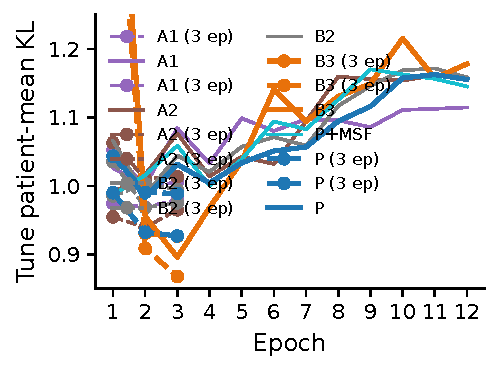
\includegraphics[width=0.95\linewidth]{figures/fig_learning.pdf}
\caption{Tune patient-mean KL per epoch for the named configurations (seed 101). Solid: 12-epoch schedule; dashed with markers: the complete 3-epoch schedule that was frozen.}
\label{fig:learning}
\end{figure}
\fi

\subsection{RQ1: primary confirmatory result}
\begin{figure}[t]
\centering
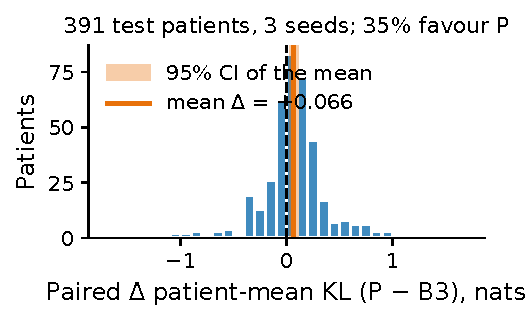
\includegraphics[width=0.95\linewidth]{figures/fig_primary.pdf}
\caption{Primary result on the locked test: per-patient paired differences in calibrated patient-mean KL (P $-$ B3, averaged over three seeds) and the 95\% bootstrap interval of their mean.}
\label{fig:primary}
\end{figure}

\begin{table*}[t]
\caption{Locked-test metrics, three-seed means. ``Cal'' = scalar temperature from Calibration-T (rank-based metrics are unchanged by a positive temperature). Hard-label metrics use the 20,482 unique-majority windows. Lower is better for KL, CE, Brier and ECE.}
\label{tab:test}
\footnotesize
\setlength{\tabcolsep}{3.5pt}
\begin{tabular}{lrrrrrrrrrrrr}
\toprule
Method & Params & Patient KL & Row KL & KL$_{\ge 10\,\text{votes}}$ & Soft CE & Brier & Macro AUROC & Macro AUPRC & Bal.\ acc. & Macro F1 & MCC & Soft ECE \\
\midrule
B3 raw & 1,524,150 & 0.943 & 0.869 & 0.754 & 1.230 & 0.592 & 0.884 & 0.656 & 0.576 & 0.580 & 0.509 & 0.107 \\
B3 cal & & \textbf{0.869} & \textbf{0.807} & \textbf{0.666} & \textbf{1.168} & \textbf{0.578} & \textbf{0.884} & \textbf{0.656} & \textbf{0.576} & \textbf{0.580} & \textbf{0.509} & \textbf{0.036} \\
P raw & 164,134 & 0.991 & 0.961 & 0.819 & 1.322 & 0.642 & 0.856 & 0.579 & 0.523 & 0.520 & 0.446 & 0.118 \\
P cal & & 0.934 & 0.906 & 0.744 & 1.267 & 0.625 & 0.857 & 0.580 & 0.523 & 0.520 & 0.446 & 0.051 \\
P+MSF cal & 208,070 & 0.958 & 0.925 & 0.738 & 1.286 & 0.634 & 0.849 & 0.561 & 0.506 & 0.502 & 0.428 & 0.040 \\
\bottomrule
\end{tabular}
\end{table*}

The hypothesis of RQ1 is rejected (Figure~\ref{fig:primary}, Table~\ref{tab:test}). With calibrated predictions $\Delta=+0.0657$, 95\% CI $\ci{+0.0334}{+0.0973}$: the candidate is inferior. The uncalibrated secondary estimate agrees ($+0.0485$, $\ci{+0.0059}{+0.0899}$). Per-seed calibrated patient-mean KL is 0.924, 0.955 and 0.924 for P and 0.878, 0.856 and 0.872 for B3; 35.3\% of patients are better predicted by the candidate. The paired standard deviation on the \ntestpat{} test patients is \testpairedsd{}, smaller than the development estimate of 0.58 because the latter was computed on 196 tune patients with checkpoint-selected 12-epoch models; at the observed spread the minimum detectable difference at 80\% power is \testmde{}, below the observed effect, so the negative result is resolved rather than under-powered. B3 leads on every secondary metric, including macro AUROC (0.884 versus 0.857) and macro AUPRC (0.656 versus 0.580). LRDA is the hardest class for both models (per-class AUROC 0.80--0.85, recall below 0.32).

\subsection{RQ2 and RQ3: mechanism ablations and confound controls}
\label{sec:ablation}
\begin{table}[t]
\caption{Post-lock development ablations under the frozen complete 3-epoch schedule (last-epoch weights, no checkpoint selection): tune patient-mean KL, mean $\pm$ SD over seeds 101/202/303, and paired within-seed differences. Test data were not used.}
\label{tab:multiseed}
\footnotesize
\setlength{\tabcolsep}{3pt}
\begin{tabular}{llrr}
\toprule
ID & Configuration & Params & Tune KL (mean $\pm$ SD) \\
\midrule
B2 & uniform, fixed fusion, no aux & 147,524 & \klBtwo{} $\pm$ \sdBtwo \\
A1 & + foveated bins & 147,524 & \klAone{} $\pm$ \sdAone \\
A2 & + learned gate & 155,877 & \klAtwo{} $\pm$ \sdAtwo \\
P & + disagreement loss & 164,134 & \klP{} $\pm$ \sdP \\
B3 & MobileNetV3-Small, ImageNet & 1,524,150 & \klBthree{} $\pm$ \sdBthree \\
B3-scratch & same, random init & 1,524,150 & \klBthreeS{} $\pm$ \sdBthreeS \\
B3-half & width 0.5, ImageNet & 574,518 & \klBthreeH{} $\pm$ \sdBthreeH \\
\midrule
\multicolumn{4}{l}{Paired $\Delta$ tune KL (mean $\pm$ SD over seeds; negative = first term better)} \\
\multicolumn{3}{l}{Foveation (A1 $-$ B2)} & \dfoveation{} $\pm$ \dsdfoveation \\
\multicolumn{3}{l}{Learned gate (A2 $-$ A1)} & \dgate{} $\pm$ \dsdgate \\
\multicolumn{3}{l}{Disagreement loss (P $-$ A2)} & \daux{} $\pm$ \dsdaux \\
\multicolumn{3}{l}{All three (P $-$ B2)} & \dall{} $\pm$ \dsdall \\
\multicolumn{3}{l}{ImageNet pretraining (B3 $-$ B3-scratch)} & \dpretrain{} $\pm$ \dsdpretrain \\
\multicolumn{3}{l}{Full vs half width (B3 $-$ B3-half)} & \dwidth{} $\pm$ \dsdwidth \\
\multicolumn{3}{l}{B3-scratch $-$ P} & \dscratchvsp{} $\pm$ \dsdscratchvsp \\
\multicolumn{3}{l}{B3-half $-$ P} & \dhalfvsp{} $\pm$ \dsdhalfvsp \\
\bottomrule
\end{tabular}
\end{table}

\begin{figure}[t]
\centering
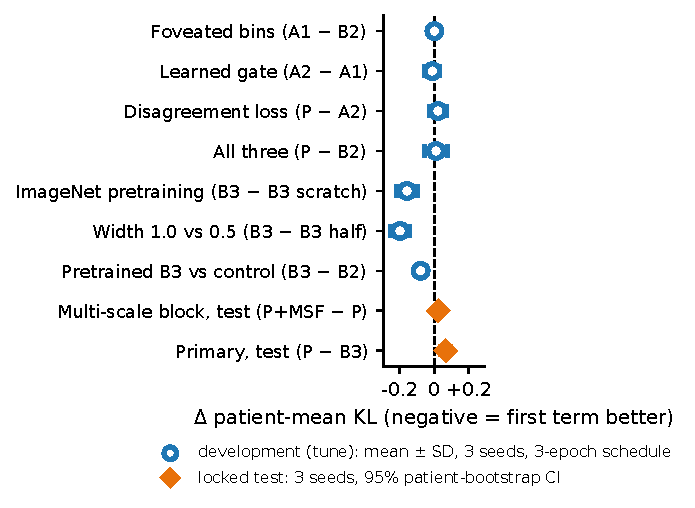
\includegraphics[width=\linewidth]{figures/fig_ablation.pdf}
\caption{Ablation ladder. Circles: post-lock development contrasts (tune, mean $\pm$ SD over three seeds, frozen schedule). Diamonds: locked-test contrasts with 95\% patient-bootstrap intervals.}
\label{fig:ablation}
\end{figure}

The single-seed development ladder of Table~\ref{tab:dev} suggested that foveation (+0.015), the learned gate ($-0.011$) and the disagreement loss ($-0.007$) barely move tune loss. Because those deltas are smaller than the seed spread observed later in the final phase, we re-ran the ladder after the lock on development data only, with three seeds under the frozen schedule (Table~\ref{tab:multiseed}, Figure~\ref{fig:ablation}). The answer to RQ2 is that none of the three mechanisms produces a benefit that exceeds seed variation: foveation changes tune KL by \dfoveation{} ($\pm$\dsdfoveation), the gate by \dgate{} ($\pm$\dsdgate) and the auxiliary loss by \daux{} ($\pm$\dsdaux); together they give \dall{} ($\pm$\dsdall). We therefore make no mechanism claim in either direction. The exploratory multi-scale block is significantly worse than P on the locked test ($+0.024$, $\ci{+0.001}{+0.045}$).

For RQ3 we trained the comparator from random initialisation (B3-scratch) and at half width with ImageNet weights (B3-half) under the same schedule and seeds. ImageNet pretraining is worth \dpretrain{} ($\pm$\dsdpretrain) tune KL and full width \dwidth{} ($\pm$\dsdwidth). Without either, the MobileNet is no longer ahead: B3-scratch is \dscratchvsp{} ($\pm$\dsdscratchvsp) \emph{worse} than P and the 575k-parameter B3-half is \dhalfvsp{} ($\pm$\dsdhalfvsp) worse, on every seed for the former. The comparator's advantage is therefore the combination of transferred features and the width those features were learned at, not a property of the inverted-residual trunk itself; a compact trunk trained from scratch on 1,170 patients is competitive with, and more stable than, an equally scratch-trained MobileNet. The candidate's own tune spread under this schedule is \sdP{}, the largest of the seven, and Section~\ref{sec:calib} traces part of it to the gate.

Inference-time modality ablation of the frozen P model on the full test (RQ4) confirms that the design uses what it claims: forcing the context path only (local view removed) raises calibrated patient-mean KL by $+0.408$ $\ci{+0.35}{+0.47}$ and flips 31.5\% of labels, whereas forcing the local path only costs $+0.090$ $\ci{+0.06}{+0.13}$; region removal costs $+0.10$ (LL), $+0.12$ (RL), $+0.20$ (LP) and $+0.07$ (RP) (Figure~\ref{fig:evidence}a). The gate's test mean is 0.45, 0.72 and 0.43 for the three seeds, so the mixture is real but seed-dependent, which is one source of the candidate's larger seed spread (SD 0.018 versus 0.011).

\subsection{RQ4: calibration, deferral and disagreement}
\label{sec:calib}
\begin{figure*}[t]
\centering
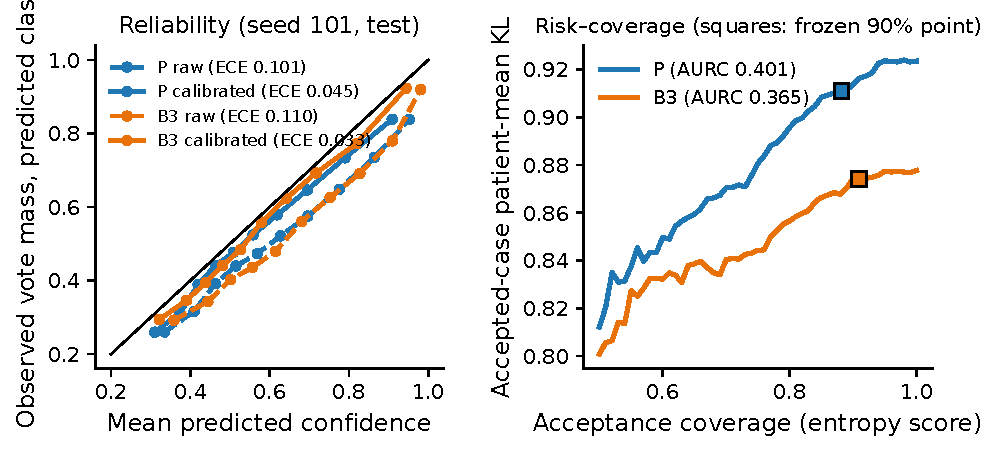
\includegraphics[width=0.84\textwidth]{figures/fig_calibration.pdf}
\caption{Left: reliability of P and B3 before and after temperature scaling (seed 101, locked test). Right: KL risk--coverage with the frozen entropy score; squares mark the operating points whose thresholds were fixed on Calibration-P.}
\label{fig:calib}
\end{figure*}
Both architectures are over-confident when trained with soft cross-entropy: temperatures fitted on Calibration-T range from 1.21 to 1.39 (P) and 1.28 to 1.33 (B3), none at a bound, and scaling cuts soft top-label ECE from 0.10--0.14 to 0.03--0.06 and patient-mean KL by 0.046--0.081 for every model and seed (Figure~\ref{fig:calib}). With entropy as the frozen score and thresholds fixed on Calibration-P, referring 11.8\% of test windows lowers P's accepted-case patient KL from 0.923 to 0.911 (seed 101); for B3, referring 9.1\% lowers it from 0.878 to 0.874. The benefit is real but modest, and the area under the risk--coverage curve is 0.401--0.415 for P against 0.365--0.372 for B3. The disagreement head predicts observed annotator disagreement with Spearman 0.31, 0.26 and 0.25 across seeds (0.23--0.24 within vote strata), but as a referral score it is worse than entropy (AURC 0.444--0.448), consistent with its target being largely a function of the primary target.

\subsection{Subgroups, robustness and evidence use}
\begin{figure}[t]
\centering
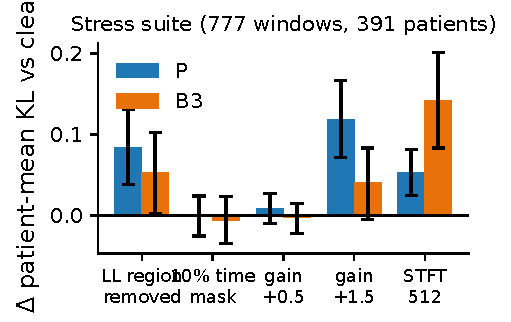
\includegraphics[width=\linewidth]{figures/fig_robustness.pdf}
\caption{Six-condition stress suite (777 label-blind test windows, 391 patients): change in calibrated patient-mean KL versus the clean input with paired patient-bootstrap intervals.}
\label{fig:robust}
\end{figure}
\begin{figure*}[t]
\centering
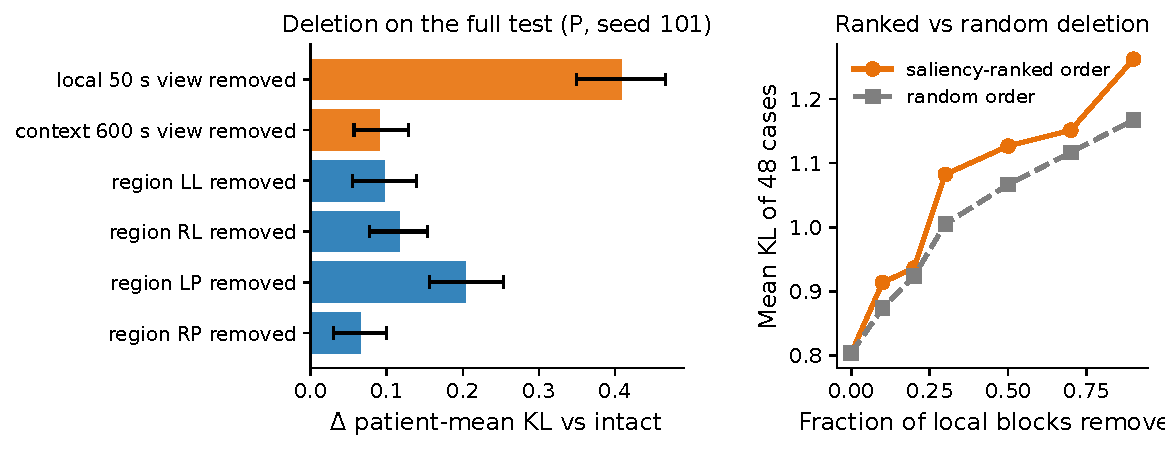
\includegraphics[width=0.84\textwidth]{figures/fig_evidence.pdf}
\caption{Evidence-use audit of the frozen P model (seed 101). (a) View and region deletion on the full test with patient-bootstrap intervals. (b) Saliency-ranked versus random deletion of local (region, time-bin) blocks on 48 prespecified cases.}
\label{fig:evidence}
\end{figure*}
Across the sixteen frozen strata (exploratory; author version appendix and repository), the comparator's advantage concentrates in confident windows and in LPD: $+0.079$ $\ci{+0.027}{+0.129}$ for windows with at least ten votes, $+0.073$ $\ci{+0.028}{+0.116}$ for unanimous windows, $+0.179$ $\ci{+0.046}{+0.308}$ for LPD-majority windows and $+0.119$ $\ci{+0.029}{+0.206}$ for windows with fewer than 95\% valid cells; on high-entropy windows ($+0.019$, $\ci{-0.033}{+0.071}$), LRDA ($-0.028$, $\ci{-0.154}{+0.093}$), GPD, GRDA, seizure and tied windows the two models are indistinguishable, and single-vote windows have low support (28 patients).

Figure~\ref{fig:robust} reports the corruption suite. Both models are insensitive to the additional time mask and to the mild gain shift. The candidate degrades three times more under a strong amplitude shift ($+0.119$ versus $+0.040$), whereas the pretrained network degrades nearly three times more under a change of STFT resolution from 256 to 512 samples ($+0.142$ versus $+0.053$), with 30\% of its labels flipping: the two families have different failure surfaces, and the second pattern is the one the preprocessing-reliability literature predicts \cite{hou2026samebrain}. Figure~\ref{fig:evidence}b shows that deleting local blocks in order of $|\nabla_x\odot x|$ raises KL faster than a random order at every fraction (1.08 versus 1.01 at 30\%), so the model's importance ranking is informative; neither fact makes it accurate.

\subsection{Resources and latency}
\ifdefined\ANONYMOUS\else
\begin{figure}[t]
\centering
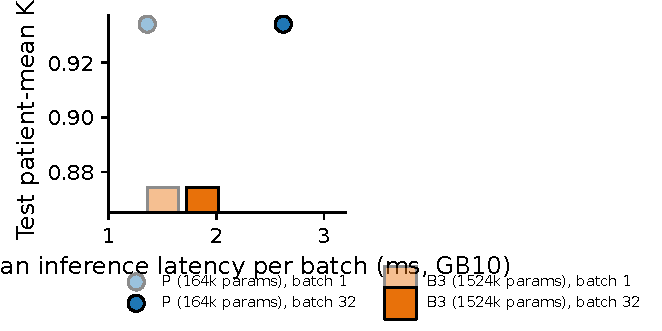
\includegraphics[width=0.95\linewidth]{figures/fig_pareto.pdf}
\caption{Calibrated test KL versus measured inference latency on the GB10 (marker area $\propto$ parameters; faint = batch 1, solid = batch 32).}
\label{fig:pareto}
\end{figure}
\fi
The locked study consumed 0.722 GPU-hours in 17 ledgered jobs with no failures (baselines 0.171\,h, ablations and pilots 0.362\,h, nine final fits 0.188\,h); the 19 post-lock development runs added 0.36\,h, for 1.08 GPU-hours in total. A final fit takes 1.11\,min (P) or 0.98\,min (B3) on the GB10 with a peak CUDA allocation of 0.44\,GiB and a process resident set of 7.6\,GiB. Cached-tensor inference has median latency 1.36\,ms at batch 1 and 2.62\,ms at batch 32 for P, and 1.50\,ms and 1.87\,ms for B3\paretoref: the batch-1 margin is within measurement noise, and at batch 32 the fused MobileNet kernels are faster despite nine times more parameters. Raw Parquet-to-prediction latency is about 45\,ms per window for both models and is dominated by I/O and the STFT. These measurements were taken on a desktop accelerator, not on an embedded device, and energy was not measured.

\section{Implementation and Reproducibility}
\label{sec:impl}
\textbf{Cache conversion} groups windows by recording, reads each Parquet file once, writes float16 values and packed masks into pre-allocated memory-mapped shards of 2,048 rows through \texttt{.partial} files renamed atomically only after both views exist for every row, and checksums each shard into a manifest; pinning BLAS to one thread per worker was necessary because multi-threaded matrix products made the context pass two orders of magnitude slower. \textbf{Training} runs under a supervisor that samples CUDA allocation, process-tree memory and system availability every fifty steps and aborts at declared stops; a \texttt{flock}-based lock forbids concurrent GPU jobs, and every job appends its wall time to the ledger whether it passed or failed. \textbf{Roles} are enforced in code: a development-role loader raises on any request for the test partition, and the evaluator role logs each test access against the protocol hash. \textbf{Release} is an allowlisted export with identifier and secret scans of the working tree and of every reachable Git object; notebooks are published with aggregate-only outputs, per-row predictions and weights stay private, and public tables suppress cells with fewer than ten patients. The repository ships 155 synthetic CPU tests, seven executed notebooks, the protocol document and twenty figures whose sidecars record the hashes they were drawn from.

\section{Discussion}
\textbf{Answers.} RQ1: no; the candidate is inferior by 0.066 patient-mean KL with an interval wholly above zero. RQ2: none of the three mechanisms improves loss beyond seed variation under the frozen schedule. RQ3: the comparator's advantage is a transfer-learning effect at full width; without ImageNet weights, or at half width, MobileNetV3-Small falls behind the candidate. RQ4: the audits show two model families that are both over-confident before scaling, both improved by entropy-based deferral, and fragile to different perturbations, with the compact model demonstrably relying on the labelled raw-EEG window.

\textbf{Why the compact candidate lost.} The task is patient-limited: 1,170 training patients contribute 64k highly correlated windows and every architecture overfits within three epochs. Under the frozen schedule the candidate ties the comparator on tune but not on the larger test, and its gate makes its seed spread 60\% larger. ImageNet features transfer to the resized two-view log-spectrogram image and are worth 0.19 KL on tune; stripped of them, or at half width, the MobileNet falls behind the compact trunk trained from scratch. The comparator's advantage is largest where evidence is clearest (unanimous or heavily annotated windows, LPD), which is where transferred texture detectors help most. The three mechanisms address problems the data do not pose: at 32 total bins the uniform encoding already resolves the 10-second centre at 1.56\,s, so the foveation null may be specific to this byte budget; the two views mostly agree, so the gate re-weights similar distributions; and the disagreement target is largely a function of the soft label already being fitted.

\textbf{Compactness is not efficiency.} A 9$\times$ smaller parameter count bought no throughput at batch 32 and only noise-level latency at batch 1, while costing accuracy and calibration against the pretrained network; it did buy accuracy and stability against the same network trained from scratch. For resource-bounded clinical inference, measured latency, memory and robustness under the deployment's own preprocessing are the quantities to report; parameter count is a poor proxy.

\textbf{Design guidance.} Cap and count the evidence so that ``compact'' is measurable; freeze the schedule rather than the checkpoint, because checkpoint selection on a tuning set overstates what a complete refit delivers; choose the comparator on data; calibrate on a partition that never trains weights and report the temperature; and audit evidence by deletion and preprocessing by perturbation, because the two audits disagreed about which model is safer.

\textbf{Threats to validity.} Only two configurations were eligible as comparator, so a stronger small network could widen the gap. The post-lock ablations are development-only and use three seeds; they cannot be confirmatory. Calibration and referral thresholds were fitted on 95 and 98 patients. The lock is self-attested through hashes and logs rather than an external registry. Subgroup contrasts are unadjusted for multiplicity.

\textbf{Limitations.} Single dataset and site; segment labels only, so no event-level sensitivity, onset latency or false-alarm rate; the disagreement statistic assumes exchangeable annotators; the corruption conditions are representation-level perturbations; single-annotator windows have noisy targets; weights are withheld pending a rights review; latency was measured on a desktop accelerator. Natural next hypotheses under a new lock are a byte-budget sweep to locate a regime in which foveation could matter, patient-level regularisation, a Dirichlet--multinomial vote model in place of the scalar disagreement head, and external validation on a second corpus.

\textbf{Data governance.} The release contains no EEG samples, spectrogram values, identifiers, split membership tables, per-window predictions or trained weights; each is reconstructible by an authorised holder of the source data from the published hashes and code. These are data-minimisation measures, not an anonymisation guarantee.

\section{Conclusion}
We asked whether byte-matched temporal foveation, a learned view gate and an annotation-disagreement auxiliary target let a 164k-parameter model match a small pretrained CNN on expert-vote EEG classification, and we specified how the question would be answered before touching the data. The answer is no. Post-lock three-seed controls show that none of the mechanisms helps beyond seed variation, and that the comparator wins through ImageNet transfer at full width rather than through its architecture: trained from scratch or at half width it falls behind the compact model. The protocol, the audits and the resource accounting are the reusable result: a complete, leak-free, audited evaluation of a clinical EEG model fits in under one GPU-hour on a single desktop accelerator, and the next attempt can start from the published lock. Code, tests, executed notebooks, the protocol document and every aggregate table are available at \repourl.

\bibliographystyle{ACM-Reference-Format}
\bibliography{refs}

\ifdefined\ANONYMOUS\else
\appendix
\section{Prespecified Subgroup Estimates}
\noindent\begin{minipage}{\columnwidth}
\captionof{table}{Paired calibrated difference in patient-mean KL (P $-$ B3, three seeds) within the sixteen strata frozen before the test; exploratory, unadjusted. Positive favours the comparator.}
\label{tab:strata}
\footnotesize
\setlength{\tabcolsep}{3.5pt}
\centering
\begin{tabular}{lrrrrl}
\toprule
Stratum & Rows & Patients & KL P & KL B3 & $\Delta$ [95\% CI] \\
\midrule
1 vote & 510 & 28 & 0.939 & 0.817 & $+0.123$ $[-0.032,+0.289]$\,$^{\dagger}$ \\
2--4 votes & 11,990 & 353 & 1.057 & 1.000 & $+0.057$ $[+0.013,+0.099]$ \\
5--9 votes & 315 & 56 & 0.491 & 0.473 & $+0.018$ $[-0.043,+0.074]$ \\
$\ge$10 votes & 8,490 & 239 & 0.744 & 0.666 & $+0.079$ $[+0.027,+0.129]$ \\
Entropy zero (unanimous) & 10,877 & 357 & 1.046 & 0.973 & $+0.073$ $[+0.028,+0.116]$ \\
Entropy middle tertile & 2,380 & 168 & 0.736 & 0.643 & $+0.094$ $[+0.051,+0.141]$ \\
Entropy upper tertile & 8,048 & 250 & 0.815 & 0.796 & $+0.019$ $[-0.033,+0.071]$ \\
Valid cells $<$ 95\% & 1,523 & 134 & 1.036 & 0.917 & $+0.119$ $[+0.029,+0.206]$ \\
Valid cells $\ge$ 95\% & 19,782 & 381 & 0.917 & 0.853 & $+0.064$ $[+0.030,+0.096]$ \\
Majority Seizure & 4,363 & 191 & 0.983 & 0.928 & $+0.056$ $[-0.007,+0.114]$ \\
Majority LPD & 2,485 & 52 & 1.171 & 0.992 & $+0.179$ $[+0.046,+0.308]$ \\
Majority GPD & 3,143 & 65 & 0.983 & 0.901 & $+0.082$ $[-0.062,+0.235]$ \\
Majority LRDA & 3,137 & 93 & 1.580 & 1.609 & $-0.028$ $[-0.154,+0.093]$ \\
Majority GRDA & 3,608 & 140 & 0.979 & 0.940 & $+0.039$ $[-0.030,+0.108]$ \\
Majority Other & 3,746 & 239 & 0.777 & 0.709 & $+0.068$ $[+0.024,+0.108]$ \\
Tied majority & 823 & 97 & 0.760 & 0.718 & $+0.042$ $[-0.021,+0.106]$ \\
\bottomrule
\multicolumn{6}{l}{$^{\dagger}$ low support (28 patients).}
\end{tabular}
\end{minipage}
\fi

\end{document}
